\chapter{Task Regrouping Framework}
\label{chap:regroup}

In this chapter, we apply on-line trace sampling(~\ref{sec:sampling})
and composable cache sharing models(~\ref{sec:iter-model}) to solve
the problem of cache conscious task regrouping.  Given a multicore
machine with $p$ processors and $c$ cores per processor, and $c \cdot
p$ tasks to execute, the goal is to divide the $c \cdot p$ tasks among
the $p$ processors to maximize the overall performance.  We present a
complete on-line setup to regroup a given set of programs for the
overall speed, which means to minimize the finish time for the longest
running task.  A similar setup may be used to maximize the throughput,
which means to minimize the average slowdown compared to running each
task in dedicated cache with no sharing. 

\section{On-line Locality Testing}
\subsection{Lifetime Sampling per Program}
\label{sec:lf-sampling}
Recall the trace sampling algorithm in
Figure~\ref{alg:fp-sampling}. Sampling is applied to average footprint
by first measuring average footprint for sampled traces and then take
the average over all the segments. In this framework, we customize the
sampling to be lifetime sampling, that is, we sample a run-time window
as long as the lifetime. Specifically, we start sampling at a random
point in execution and continue until the program accesses as much
data as the size of the cache. 

Similar to the sampling introduced in Figure~\ref{alg:fp-sampling},
lifetime sampling takes a sample every $k$ seconds for a lifetime
window for cache size $c$. When a program starts, we set the system
timer to interrupt every $k$ seconds. The interrupt handler forks a
sampling task and attaches the binary rewriting tool
Pin~\cite{Pin:PLDI05}.  The Pin tool instruments the sampling process
to collect its data access trace, measures all-window footprint using
our technique described in~\ref{sec:avg-fp}, and finds the
lifetime $lf(c),lf(c+1)$.  

For in situ testing, we do not increase the number of tasks.  The
sampling algorithm ensures this in two ways.  First, the sampling task
does not run in parallel with the base task.  This is done by the base
task waiting for the sampling task to finish before continuing.
Second, no concurrent sampling is allowed.  Timer interrupt is turned
off for the sampling task.  The base task sets a flag when a sampling
task is running and ignores the timer interrupt if the flag is up.

\paragraph{Comparison with reuse-distance sampling}
Lifetime by definition is more amenable to sampling.  We can start a
lifetime sample at any point in an execution and continue until the
sample execution contains enough access to fill the size of target cache.
We can sample multiple windows independently, which means they can be
parallelized.  It does not matter whether the sample windows are
disjoint or overlapping, as long as the choice of samples is random
and unbiased.  In contrast, reuse distance sampling must sample evenly
for different lengths of reuse windows.  When picking an access, it
needs to measure the distance to the next reuse.  Since most reuse
distances are short, we have to pick more samples.  When a reuse
distance is long, we do not know a priori how long so we need to keep
analyzing until seeing the next reuse.  Therefore, reuse distance
sampling is more costly than lifetime sampling because it needs more
samples and longer samples (a reuse window can be arbitrarily longer
than a lifetime window). 


\subsection{Predicting the Miss Rate}
With trace fastly sampled, we are able to compute footprint in linear
time and derive other useful metrics, such as reuse distance,
immediately with our higher older theory of locality(\ref{chap:model}). 
For each sample $x_i$, we predict the miss rate function $mr(x_i, c)$
for each cache size $c$ with the following steps.

\begin{enumerate}
\item Use average footprint analysis(\ref{sec:avg-fp}) to compute
  the average footprint function $\overline{fp}$.  
\item Compute reuse distance distribution by the conversion from
  footprint provided by the higher order theory of locality.
\item Use reuse distance distribution and the Smith
  formula~\cite{Smith:ICSE76} to estimate the number of conflict
  misses for given cache associativity and cache size. 
\end{enumerate}

\subsection{Group Sampling per Phase}
A phase is a unit of time that co-run tasks are regrouped once.
Group sampling proceeds in phases.  It solves two problems.  First, a
program collects and analyzes one and only one lifetime sample (trace)
in each phase.  Second, when all programs have finished
sampling, the regrouping routine is called to
process the sample results and reorganize the co-run tasks (see the next
section).

We use shared memory to coordinate but do so in a distributed fashion
without a central controller.  When started, each program connects to
shared memory of a preset identifier and allocates this shared memory
if it is the first to connect.  The shared memory contains a sample
counter initialized to the number of co-run tasks and a phase counter
initialized to 0.  When a program finishes collecting a sample, it
decrements the sample counter.  The last program to finish sampling
would reduce the sample counter to 0.  It would call the regrouping
routine, reset the sample counter, and advance the phase counter.
With the two counters, the tasks would sample once and only once in
each phase.  The pseudo code is shown in Figure~\ref{alg:phase_control}.

\medskip
\begin{figure}[h!]
 \centering
 \small
 \begin{minipage}{\linewidth}
   \begin{algorithmic}[1]
     \REQUIRE group sampling, coordinated using shared memory
     \STATE \COMMENT{when a program starts}
     \STATE connect to shared memory
     \IF { shared memory not exists}
        \STATE allocate shared memory
        \STATE $count \gets 8$
        \STATE $phase\_count \gets 0$
     \ENDIF
     \STATE \COMMENT{when a program finishes a sample}
     \STATE lock shared memory
     \STATE $count \gets (count - 1)$
     \IF {$count == 0 $}
         \STATE call the regrouping routine
         \STATE $count \gets 8$
         \STATE $phase\_count \gets (phase\_count+1)$
     \ENDIF
     \STATE unlock shared memory
   \end{algorithmic}
   \caption{Group sampling per phase}
   \label{alg:phase_control}
 \end{minipage}
\end{figure}

\section{Dynamic Regrouping}

We use the following terms.  A \emph{peer group} is a set of programs
that share cache.  A \emph{configuration} (or \emph{grouping}) of a
set of programs is one way to divide the programs into peer groups.
Two groupings differ if their peer groups are not all identical.

The regrouping algorithm is shown in two parts. The first part, shown in
Figure~\ref{alg:feet}, takes the sample results, predicts and ranks
the performance of all groupings. In this algorithm, we assume that
the machine in use is a multicore machine with 2 processors and 4
cores per processor. Our algorithm can be easily generalized to $m$
processors and $n$ cores per processor, where $m$ and $n$ are positive
integers. We further assume that the first peer group, denoted by
$s_1$, includes four programs run on the first processor, and the
second peer group, denoted by $s_2$, includes the other four programs
run on the second processor. The eight programs are denoted as $p_0, p_1, ..., p_7$. 

\medskip
\begin{figure}[h!]
 \centering
 \small
 \begin{minipage}{\linewidth}
   \begin{algorithmic}[1]
     \REQUIRE regrouping routine, called when all
       programs finish sampling for the current phase.
     \STATE $d_{old}$ is the previous grouping
     \FOR {each $prog$}
        \STATE $fp[prog] \gets$ average footprint curves for $prog$
        \STATE $rd[prog] \gets$ reuse distance computed from $fp[prog]$
     \ENDFOR
     \FOR {each even division $d_i=\{s_1, s_2\}$}
        \FOR {$p_i$ in $s_1=[p_0, p_1, p_2, p_3]$}
           \STATE $mr[p_i] \gets$ shared cache miss rate from 
           \STATE \indent \indent ($rd[p_i]$, $fp[p_{j}\|p_{j} \in s_1, j \ne i]$)
           \STATE $runtime[p_i] \gets$ time\_model($mr[p_i]$)
        \ENDFOR
        \FOR {$p_i$ in $s_2=[p_4, p_5, p_6, p_7]$}
           \STATE $mr[p_i] \gets$ shared cache miss rate from 
           \STATE \indent \indent ($rd[p_i]$, $fp[p_{j}\|p_{j} \in s_2, j \ne i]$)
           \STATE $runtime[p_i] \gets$ time\_model($mr$[$p_i$])
        \ENDFOR
        \STATE $time[d_i] = \max(\ runtime[p_j\| 0 \le j \le 7])$
     \ENDFOR
     \STATE find $d_{new}$, where $time[d_{new}] \le time[d_{j, 0\le j \le 34}]$
     \STATE call the remapping routine
     \STATE $d_{old} = d_{new}$
   \end{algorithmic}
   \caption{The regrouping routine to select the grouping that
     minimizes the slowest finish time.}
   \label{alg:feet}
 \end{minipage}
\end{figure}

Once a new grouping is selected, we need to move programs between
peer groups.  Program migration incurs two types of overheads.  The
first is the direct cost of migration, including the OS delay and
re-warming of the cache.  The second is the indirect cost that happens on
machines that have NUMA memory.  When a program is started, its
data is allocated in the close-by memory module.  Migration would lose
the processor-memory affinity and cause memory access to incur additional
latency.

For these reasons, we use a remapping routine, shown in
Figure~\ref{alg:remapping}, to minimize the number of cross-processor
program migration. The routine takes the old grouping and new
grouping as the inputs, figures out the minimum process moves to
switch from old grouping to new grouping. Specifically, it compares
the peer groups in the old and the new groupings.  If we assume two
peer groups per grouping, we simply check which group assignment has
fewer migrations and choose that one. 


\medskip
\begin{figure}[h!]
 \centering
 \small
 \begin{minipage}{\linewidth}
   \begin{algorithmic}[1]
     \REQUIRE remapping routine, called after the regrouping routine
     to implement the regrouping with minimal cross-socket task migration.
     \STATE INPUTS: $d_{old}=\{s1_{o}, s2_{o}\}$, $d_{new}=\{s1_{n}, s2_{n}\}$
     \STATE $half = s1_{o}$
     \STATE $list_1 \gets (half - s1_{n})$
     \IF {$list_1$ has more than 2 elements}
        \STATE $half = s2_{o}$
        \STATE $list_1 \gets (half - s1_{n})$
     \ENDIF
     \STATE $list_2 \gets (s1_{n} - half)$
     \FOR {($p_i, q_i$) where $p_i$ and $q_i$ are the i-th elements in $list_1$ and $list_2$ correspondingly}
        \STATE swap $p_i$ and $q_i$
        \STATE update the cpu id for $p_i$ and $q_i$
     \ENDFOR
   \end{algorithmic}
   \caption{The remapping routine that minimizes the number of
     cross-processor program migration.}
   \label{alg:remapping}
 \end{minipage}
\end{figure}

To simplify the demonstration, we suppose There are
only two cores, each has 4 CPUs. $s1$ and $s2$ are the sets of
processes run on two cores correspondingly. The subscript $o$ and $n$
represents old grouping and new grouping correspondingly. Since each
set has 4 processes, there are at most 2 moves for any possible
grouping changes. The processes are moved with system command
$taskset$. The CPU id's for each processes are also updated to track
the migrations. 


\section{Evaluation}

\subsection{Target Machine and Applications}
\label{sec:eval_setup}

We test our framework of task regrouping on a machine with two Intel
Nehalem quad-core processors. Each socket has four 2.27GHz cores
sharing an 8MB L3 cache. Private L1 and L2 cache are 32KB and 256KB
respectively. The machine organizes the main memory in a NUMA
structure, and each processor has 4GB 1066MHz DDR3 memory local to
it. The machine is installed with Fedora 11 and GCC 4.4.1. 

To create a parallel workload, we select the test programs from the
SPEC 2006 benchmark suite.  To fairly evaluate co-run choices by the
longest finish time, we select the programs that have a similar
execution time when running by itself on our test machine.  
 
We have selected 12 programs shown in Table~\ref{tbl:bench}.  The
targeted time for the stand-alone execution is around 10 minutes.  
We adjusted the input for several programs to nudge their
run time closer to the target.  The stand-alone run time ranges from
530 seconds to 704 seconds for the 8 floating-point programs, shown in
the two leftmost groups, and from 459 seconds to 693 seconds for the 4
integer programs, shown in the rightmost group.

\begin{table}[h]
\centering
\small
\begin{tabular}{|l|c|c|c|c|c|}
\hline
benchmark & time & benchmark &time & benchmark & time \\
(fp) &(sec.)& (fp) &(sec.) & (int) &(sec.)\\ \hline \hline
433.milc & 530 &436.cactus &617& 401.bzip2&613 \\ \hline
434.zeusmp &704 &450.soplex &626& 429.mcf&459 \\ \hline
437.leslie3d &555& 459.Gems &629& 458.sjeng&644 \\ \hline
444.namd &608& 470.lbm &648& 462.libquan&693 \\ \hline
\end{tabular}
\caption{Benchmark statistics}
\label{tbl:bench}
\end{table}

We form two workloads from the 12 programs, each with 8 programs. The
leftmost 8 programs in Table~\ref{tbl:bench} form the floating-point
workload.  The rightmost 8 programs form the mixed workload with both
floating-point and integer code.  The middle 4 floating-point programs
are shared in both workloads.

%\newlength{\wid}
%\setlength{\wid}{8.7cm}
\begin{figure}[h]
\centering
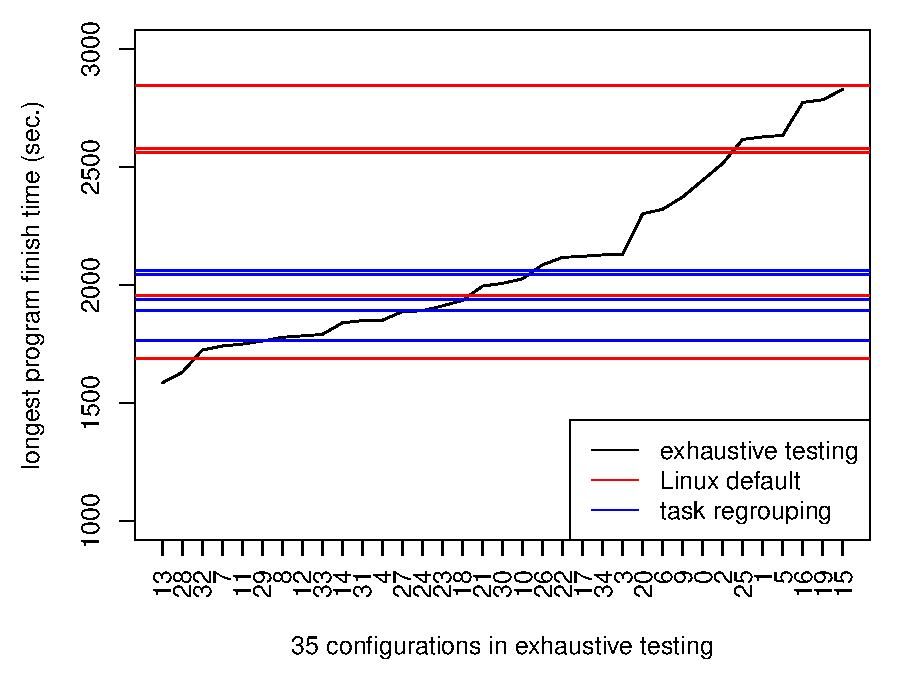
\includegraphics[width=0.45\textwidth]{figures/regroup/mix_max.pdf}
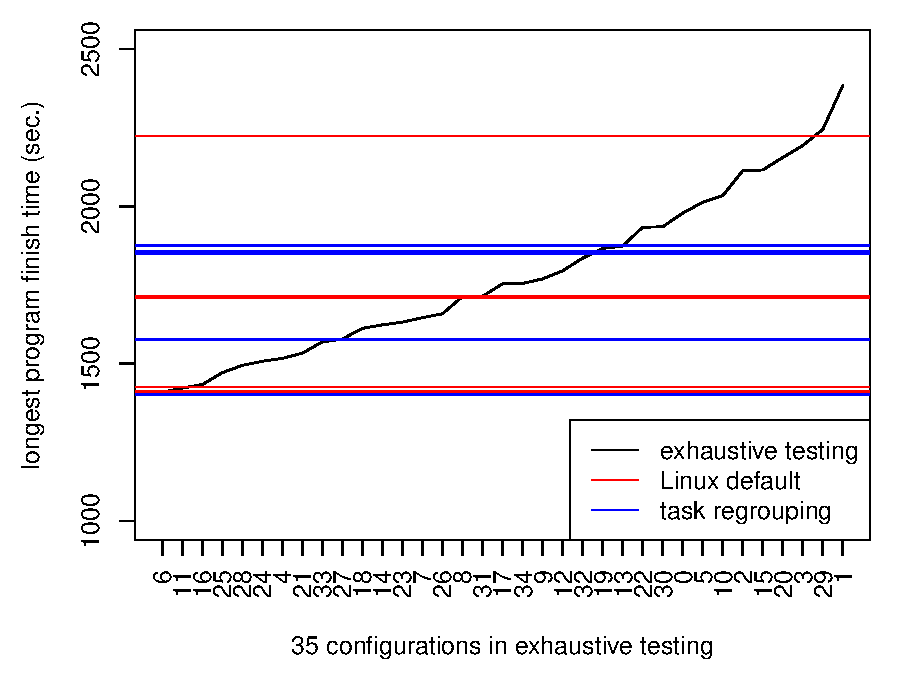
\includegraphics[width=0.45\textwidth]{figures/regroup/fp_max.pdf}
\caption{Max-time co-run graphs to compare cache-conscious task
  regrouping with default Linux scheduling and exhaustive
  testing. (Left) Mixed floating-point and integer workload.  (Right)
  Floating-point only workload.  The choice selected by task
  regrouping is grouping 27 in both workloads. }
\label{fig:max}
\end{figure}

\newlength{\height}
\setlength{\height}{8.5cm}
\begin{figure}[h]
\centering
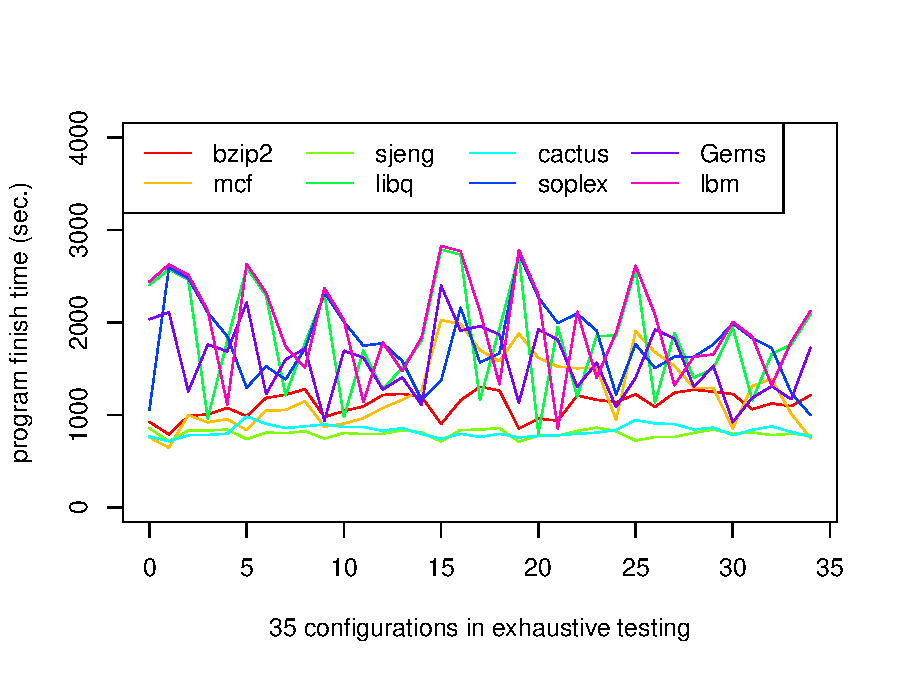
\includegraphics[width=0.45\textwidth,height=\height]{figures/regroup/mix_static.pdf}
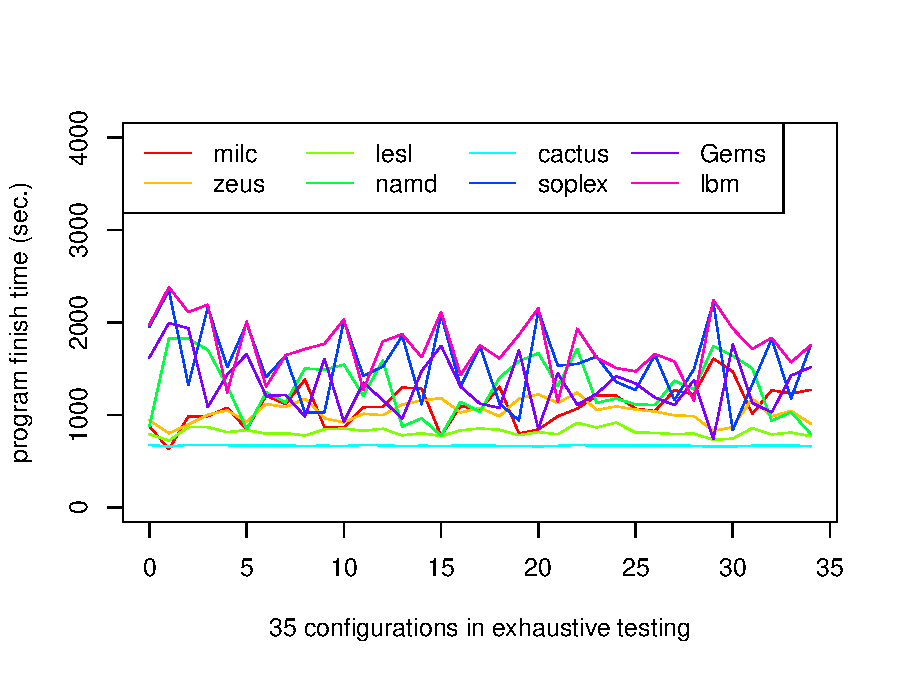
\includegraphics[width=0.45\textwidth,height=\height]{figures/regroup/fp_static.pdf}
\caption{All-time co-run graphs.  (Left) Mixed floating-point and
  integer workload.  (Right) Floating-point only workload.  The choice selected by task
  regrouping is grouping 27 in both workloads.  }
\label{fig:all}
\end{figure}

\subsection{Effect of Task Regrouping}

We compare co-run results in two types of graphs.  The first plots the
finish time of the longest running program in each grouping.  The
$x$-axis enumerates all groupings, and the $y$-axis shows the slowest
finish time.  We call it a \emph{max-time co-run graph}.  For our tests,
the $x$-axis has 35 points for the 35 groupings of 8 programs on two
quad-core processors.  

The second type of graphs also enumerate all groupings
along the $x$-axis, but the $y$-axis shows the finish time for all
the programs.  We connect the points of each program in a line.  We
call it an \emph{all-time co-run graph}.  For our tests, there are 8
lines each connecting 35 points in an all-time graph.

\paragraph{The effect of cache sharing}
The main results are shown by the two max-time co-run graphs in
Figure~\ref{fig:max}.  The max finish time for all groupings are
sorted from shortest to longest.  We see that multicore program
co-runs have a significant impact in single-program performance.  For
the mixed workload, the longest execution when running alone is 693
seconds.  In the 8-program co-run, the shortest time to finish is 1585
seconds, and the longest 2828 seconds.  The results show
the strength and the weakness of the multicore architecture. 
The single-program speed is lower, but the throughput is higher.
Cache-conscious scheduling is important because it may improve
single-program speed from 24\% to 43\% of the sequential speed and the
parallel throughput from 200\% to 350\% of the sequential throughput. 

The potential benefit is equally significant for the floating-point
workload.  The longest stand-alone time is 704 seconds.  For the
35 co-runs.  Cache-conscious scheduling may improve single-program
speed from 30\% to 50\% of the sequential speed and the parallel
throughput from 200\% to 340\% of the sequential throughput. 

The difference between the best and the worst co-run performance is
78\% for the mixed workload and 69\% for the floating-point workload.
The choice of task grouping is highly important, considering that the
potential improvement is for each of the 8 programs, not just a single
program. 

\paragraph{Task regrouping for the mixed workload}
We tested five runs of task regrouping and five runs of the default
Linux scheduling and show the 10 finish times as 10 horizontal lines
in the left-hand side graph in Figure~\ref{fig:max}.  Default Linux
times, plotted in red, are 1687, 1955, 2560, 2578, and 2844 seconds.  Task
regrouping times, plotted in blue, are 1764, 1892, 1939, 2043, and
2059 seconds.  If we take the geometric mean (to reduce the effect of
outliers), the average finish time in the five runs is 2282 seconds
for Linux and 1937 for task regrouping.  The improvement is 18\%.

In addition to being on average faster, the performance variation 
is smaller from run to run when using task regrouping.  The
difference between the largest and the smallest numbers in the five 
runs are 1157 seconds for Linux and 295 seconds for task
regrouping, a reduction by a factor of nearly 4(3.9).  

Task regrouping chooses the same grouping in every run.  Its
performance varies for two reasons.  The first is that the current
system stops regrouping once one of the 8 programs finishes.  The
remaining period is at the whim of the default Linux scheduler.  The
second is the processor-memory affinity, which depends on the initial
configuration that varies from run to run.

The all-time co-run graph in Figure~\ref{fig:all} shows how
individual programs are affected by the program co-run.  The groupings
are not sorted in the graph.  We see that the speed of some programs, in
particular \emph{cactus} and \emph{sjeng}, does not vary with the co-run
peers (even though the co-run speed is significantly slower
than stand alone).  The speed of other programs, in particular \emph{lbm},
\emph{libq}, and \emph{soplex}, vary by a factor of 2 in performance
depending on who their peers are.

The task regrouping chooses grouping 27, which includes \emph{lbm,
  soplex, sjeng, bzip2} in one peer group and the rest in the other
peer group.   Each peer group has two floating-point and two integer
programs.  

\paragraph{Task regrouping for the floating-point workload}
For the floating-point workload, task regrouping does not improve the
average finish time.  Default Linux runs finish in 1412, 1426, 1709,
1713, and 2223 seconds.  Task regrouping runs finish in 1403, 1576,
1850, 1857, and 1874 seconds.  The geometric mean is 1673 seconds for
Linux and 1701 seconds for task regrouping.  The latter is 1.7\%
slower.  However, task regrouping has much smaller variation.  The
largest difference between the five runs is 811 seconds for Linux and
471 seconds for regrouping.  The latter is a factor of 1.7 smaller.

The regrouping chooses also grouping 27, which includes
\emph{lbm,milc,leslie3d,namd} in one peer group and the rest in the
other peer group.  The relatively poor result is partly due to the
accuracy of the model and partly due to overhead of sampling, which we
discuss next.

\subsection{Overhead of On-line Sampling}

Sampling has a direct overhead, because it pauses the base program,
and an indirect overhead, because it adds to cache interference and
competes for other resources such as memory bandwidth.  We
have measured the first overhead.  Tables~\ref{tbl:mix_overhead}
and~\ref{tbl:fp_overhead} show for each program, the total length of
the sampling pause as a portion of the total length of the co-run
execution. 

In the mixed workload, the top three overheads are 18\%, 14\%, and
5\%.  The rest are between 0.9\% and 1.3\%.  In the floating-point
workload, all overheads are below 1\% except for \emph{cactus} 21\%
and \emph{namd} 31\%.  The \emph{namd} cost is likely a main reason
for the relatively poor performance of task regrouping for the
floating-point workload.  

\begin{table}[t!]
\centering
\small
\begin{tabular}{|l|c|c|c|}
\hline
benchmark & overhead (\%) & benchmark & overhead (\%) \\ \hline \hline
436.cactus &18.0& 401.bzip2&13.7 \\ \hline
450.soplex &1.3& 429.mcf&1.2 \\ \hline
459.Gems &1.3& 458.sjeng&5.1 \\ \hline
470.lbm &0.9& 462.libquan&1.1 \\ \hline
\end{tabular}
\caption{Sampling overhead when regrouping for the mixed
  floating-point and integer workload}
\label{tbl:mix_overhead}
\end{table}

\begin{table}[t!]
\centering
\small
\begin{tabular}{|l|c|c|c|}
\hline
benchmark & overhead (\%) & benchmark & overhead (\%) \\ \hline \hline
433.milc & 1.0 &436.cactus &21.1 \\ \hline
434.zeusmp &0.6 &450.soplex &0.2 \\ \hline
437.leslie3d &0.1& 459.Gems &0.3 \\ \hline
444.namd &31.2& 470.lbm &0.1 \\ \hline
\end{tabular}
\caption{Sampling overhead when regrouping for the floating-point workload}
\label{tbl:fp_overhead}
\end{table}

\section{Discussion}
In this chapter, we have proposed a framework of cache-conscious task
regrouping. This is a system that integrates our previously introduced
techniques, trace sampling, higher order theory of locality, and
offline cache interference prediction. It combines the strength of
both online and offline models and provides accurate performance
predictions. In this work, we consider only parallel workloads of
independent sequential programs.  Multi-threaded workloads pose the
additional problems of data and code sharing and thread interleaving,
which we will consider in future work.  
